%        File: L3.tex
%     Created: mer. nov. 23 06:00  2016 C
% Last Change: mer. nov. 23 06:00  2016 C
%
\documentclass[a4paper]{article}

\usepackage[utf8]{inputenc}
\usepackage[T1]{fontenc}
\usepackage[french]{babel}
\usepackage{verbatim}
\usepackage{graphicx}
\usepackage[margin=2cm]{geometry}
\usepackage{amssymb}
\usepackage{caption} 

\title{Rapport Niveau 3 – PS5 BRAINF-CK}
\author{MIAOU – MIAOU Is An Open Umbrella\\
Nassim BOUNOUAS - Guillaume CASAGRANDE \\ Julien LEMAIRE - Pierre-Emmanuel NOVAC}

\begin{document}

\maketitle

\section{Introduction}
\paragraph{}Nous vous présentons à travers ce rapport notre version de l'interpréteur du langage de programmation exotique \textsc{Brainf*ck} développée à ce jour jusqu'à la fin du niveau 3, suivant le découpage du sujet d'origine. Nous avons donc repris les fonctionnalités dont le développement a été achevé dans les deux précédents niveaux, à savoir :
\begin{itemize}
	\item La mise en place d'une \texttt{Machine} virtuelle et d'une mémoire (\texttt{Memory}).
	\item Le support des différentes \texttt{Instruction}s proposée par le langage \textsc{Brainf*ck} (\texttt{INCR}, \texttt{DECR}, \texttt{LEFT}, \texttt{RIGHT}, \texttt{IN}, \texttt{OUT}, \texttt{JUMP}, \texttt{BACK}).
	\item La redirection des flux d'entrée et de sortie pour que les instructions \texttt{IN} et \texttt{OUT} puissent respectivement lire et écrire dans des fichiers plutôt que sur l'entrée/la sortie standard.
	\item Le support des sauts conditionnels dans une implémentation naïve (décrite plus tard) et de la vérification de leur bonne utilisation dans un programme donnée.
	\item Le support des différentes syntaxes décrites dans le sujet, à savoir la syntaxe image (les instructions étant alors codées sous la forme de couleurs de 3 x 3 pixels), la syntaxe texte dite ``longue'' (les instructions sont alors écrites ligne par ligne, sous la forme de leur nom suscité) et la syntaxe texte dite ``courte'' (la syntaxe la plus connue, agrémentée de symboles).
	\item Le module de traduction (\texttt{Translator}) afin de pouvoir passer d'une syntaxe à une autre.
\end{itemize}
\paragraph{}Ces fonctionnalités étant implémentées, nous devions alors y rajouter celles du niveau 3. Celles-ci étaient, entre autres, composées des \texttt{Metrics} qui, à chaque lancement d'un programme \textsc{Brainf*ck}, propose des données sur son exécution, ou encore du \texttt{Logger} qui, à la demande de l'utilisateur, devait fournir un fichier log, lié au programme exécuté, et détaillant les différentes instructions effectuées avec leur conséquence propre sur la \texttt{Machine} et la \texttt{Memory}. Le support des commentaires et de l'indentation permettaient de rentre un programme \textsc{Brainf*ck} aussi libre et compréhensible que l'auteur l'eusse souhaité.
\paragraph{}En dehors de ces outils, plus de l'ordre de la maintenance d'un programme \textsc{Brainf*ck} et de sa clarté, l'ajout du support des \texttt{Macros} était réellement une vraie fonctionnalité supplémentaire pour le développeur \textsc{Brainf*ck}, qui pourrait alors sauvegarder un morceau de code sous l'appellation de son choix. Chaque appel de cette même appellation serait alors remplacé par le code lui-même lors de la lecture du fichier. Enfin, la \texttt{JumpTable} est apparue comme une amélioration potentiellement considérable de notre implémentation naïve des sauts conditionnels, permettant de lier chaque instruction \texttt{JUMP} à l'instruction \texttt{BACK} associée et inversement.
\paragraph{}Proposer une implémentation de ces différentes fonctionnalités était donc notre objectif pour terminer ce niveau 3. Cet objectif étant à présent atteint, nous vous présenterons dans ce rapport nos différents choix d'implémentations pour le réaliser.

\section{Nos choix d'implémentations}

\subsection{Schéma d'implémentation / Diagramme de classes}
\paragraph{}La \textsc{Figure 1} décrit une vision globale de l'architecture de notre application en termes de classes, de fonctionnalités et d'interaction entre les classes. Certains détails de ce diagramme seront abordés plus amplement par la suite.
\begin{center}
	\includegraphics[scale=0.7]{pres23.png}
	\captionof{figure}{Diagramme de classes}
\end{center}

\subsection{Metrics}
\paragraph{}Comme précisé en introduction, les \texttt{Metrics} sont des données fournies à chaque interprétation d'un programme \textsc{Brainf*ck} à propos de celui-ci et de son exécution. Ces \texttt{Metrics} sont composés de 6 valeurs, à savoir :
\begin{itemize}
	\item \texttt{PROG\_SIZE}, qui contient le nombre d'instructions écrites dans le programme interprété.
	\item \texttt{EXEC\_TIME}, qui donne le temps d'exécution du programme en ms.
	\item \texttt{EXEC\_MOVE}, qui donne le nombre de fois que le pointeur d'exécution (entendons par là, le pointeur sur les instructions à exécuter) a été déplacé.
	\item \texttt{DATA\_MOVE}, qui donne le nombre de déplacements du pointeur sur la mémoire lors de l'exécution du programme.
	\item \texttt{DATA\_READ}, qui donne le nombre d'opérations de lecture de la mémoire effectuées par le programme.
	\item \texttt{DATA\_WRITE}, qui donne le nombre d'opérations d'écriture dans la mémoire effectuées par le programme.
\end{itemize}

\paragraph{}Ces \texttt{Metrics} sont systématiquement affichés à la fin de l'exécution d'un programme \textsc{Brainf*ck}, comme le décrit la \textsc{Figure 2} :
\begin{center}
	\includegraphics[scale=0.35]{metrics.png}
	\captionof{figure}{Affichage des \texttt{Metrics} à la fin de l'exécution d'un programme \textsc{Brainf*ck}}
\end{center}

\paragraph{}D'un point de vue implémentation, les différentes \texttt{Metrics} sont tout simplement stockées dans un \texttt{enum}. Chacun des éléments de cet \texttt{enum} (nommé \texttt{Metrics}) possède un attribut de type \texttt{long}. Il peut être modifié par diverses méthodes. Ainsi, on peut l'incrémenter, via une méthode nommée \texttt{incr}, ou encore directement changer sa valeur en dur par le biais d'une méthode \texttt{set} ou finalement l'utiliser comme un chronomètre avec les méthodes \texttt{start} et \texttt{stop}. Cette pluralité dans les moyens de modifications des \texttt{Metrics} sert bien sur à couvrir  tous les comportements possibles (chacune d'entre elles ne se calculant pas de la même façon, \texttt{EXEC\_TIME} est le seul calculateur de temps par exemple). Toutefois, nous reconnaissons que cette implémentation pose le problème de la liberté du changement de valeur. Il est possible ici de calculer \texttt{DATA\_WRITE} comme un temps par exemple alors que cela devrait être impossible. Nous avions réfléchi à une meilleure implémentation, plus orientée objet, pour régler ce problème, mais la solution de l'\texttt{enum} s'imposait comme la plus simple malgré tout.

\paragraph{}Nous avons choisi de diviser les différentes \texttt{Instructions} que propose le langage \textsc{Brainf*ck} en différentes catégories. Pour rappel, nous avions implémenté ces \texttt{Instructions} sous la forme d'un Command Pattern, c'est-à-dire qu'elles héritaient toutes d'une classe mère \texttt{Instruction} définissant une méthode nommée \texttt{accept}. Cette méthode est alors surchargée dans les classes filles pour définir le comportement d'une instruction donnée sur la \texttt{Machine} et la \texttt{Memory}.

\paragraph{}Ces mêmes \texttt{Instructions} influent sur une partie des \texttt{Metrics}, chacune augmentant précisément l'une d'entre elles à chacune de leurs exécutions. En l'occurrence :
\begin{itemize}
	\item \texttt{Left} et \texttt{Right} influent sur \texttt{DATA\_MOVE}.
	\item \texttt{In}, \texttt{Incr} et \texttt{Decr} influent sur \texttt{DATA\_WRITE}.
	\item \texttt{Out}, \texttt{Jump} et \texttt{Back} influent sur \texttt{DATA\_READ}.
\end{itemize}
\paragraph{}Ces comportements communs entre les différentes instructions nous ont conduits à la création de classes mères de façon à les séparer en fonction de leurs agissements sur les \texttt{Metrics}. Elles implémentent donc ces comportements dans leur méthode \texttt{accept} à laquelle les classes filles font appel dans leur propre méthode \texttt{accept}. Nous avons donc créé les classes \texttt{MoveCursor}, \texttt{ReadMemory} et \texttt{WriteMemory} et les instructions suivent désormais l'architecture décrite dans la \textsc{Figure 3}.
\begin{center}
	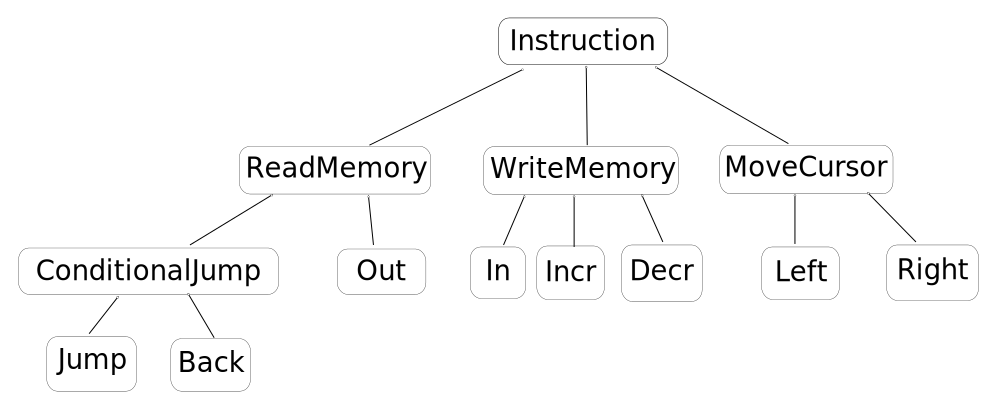
\includegraphics[scale=0.4]{schemametrics.png}
	\captionof{figure}{Architecture des \texttt{Instructions} en prenant en compte les \texttt{Metrics}.}
\end{center}
\paragraph{}Si ce choix peut paraitre compliqué pour un simple changement de valeur, il permet de regrouper par l'héritage des comportements communs, plutôt que de recopier ce même comportement dans plusieurs classes différentes. Ainsi, si le code de modification des \texttt{Metrics} se voit être complexifié par l'avenir, il pourra être plus facilement modifiable du point de vue des instructions.

\paragraph{}Pour ce qui est des \texttt{Metrics} restantes, elles sont toutes modifiées au sein même de l'\texttt{Interpreter}. \texttt{PROG\_SIZE} est directement mise à la valeur de la taille de la liste d'instructions tandis qu'\texttt{EXEC\_TIME} calcule la différence de temps entre le début et la fin de la boucle d'exécution du programme. Enfin, \texttt{EXEC\_PROG} est incrémentée à chaque tout d'exécution de la boucle (le pointeur d'exécution ayant nécessairement bougé à chaque fois d'une case). La modification de ces \texttt{Metrics} est ainsi centralisée et peut être facilement modifiée. La nouvelle boucle d'exécution de l'\texttt{Interpreter} peut ainsi être représentée par le morceau de code suivant :
\begin{verbatim}
int i = 0;
		Metrics.PROG_SIZE.set(instructions.size());
		Metrics.EXEC_TIME.start();
		while (i >= 0 && i < instructions.size()) {
		    //old interpreting stuff
		    Metrics.EXEC_MOVE.incr();
		    i++;
		}
		Metrics.EXEC_TIME.stop();
\end{verbatim}

\subsection{Logs}
\paragraph{}Les logs sont des fichiers retraçant le déroulement de l'exécution d'un programme \textsc{Brainf*ck}. Ils restituent ainsi un certain nombre d'informations récoltées lors de l'exécution de chaque \texttt{Instruction} spécifiée dans le programme \textsc{Brainf*ck}. Un fichier log est créé à chaque fois que l'exécutable de notre application est appelé avec l'option \texttt{--trace}, conformément aux spécifications.

\paragraph{}La création du fichier de log est alors géré par une classe nommée \texttt{Logger}. Un objet \texttt{Logger} est créé avec comme paramètre le nom du fichier \textsc{Brainf*ck} actuellement exécuté (qu'il soit sous format texte ou image), ceci dans le but de pouvoir remplacer l'extension du fichier par « \texttt{.log} », ce qui nous donne le nom de notre futur fichier de log. Ces opérations sont exécutées dans le constructeur et non pas depuis l'extérieur de la classe, ce qui permet réellement d'isoler ce comportement spécifique au \texttt{Logger}. Ceci augmente donc son indépendance vis à vis des autres classes, autrement dit, cela diminue le « coupling » général du programme.

\paragraph{}En ce qui concerne l'écriture du fichier lui-même, le \texttt{Logger} possède un attribut de type \texttt{WriteTextFile} associé au nom de fichier construit précédemment. En conséquence, la classe implémente une méthode \texttt{logstep} qui, à chaque appel, écrit une nouvelle étape de log dans le fichier prévu à cet effet. Un tel ajout contiendra un certain nombre d'informations, à savoir :
\begin{itemize}
	\item Le numéro de l'\texttt{Instruction} exécutée, défini par incrémentation (première valeur égale à 1).
	\item L'emplacement du pointeur d'exécution (pour rappel, le pointeur parcourant les instructions à exécuter).
	\item Le nom de l'\texttt{Instruction} exécutée (sous la forme de sa représentation en syntaxe longue (INCR par exemple)).
	\item L'emplacement du pointeur de données (la case mémoire sur laquelle on travaille).
	\item Un affichage entier de la mémoire après exécution de l'instruction.
\end{itemize}

\paragraph{}En outre, une étape de log s'affichera comme suit dans le fichier correspondant :
\begin{verbatim}
21 — exec 11: INCR on C0
C0: 1
C1: 53
\end{verbatim}

\paragraph{}La méthode \texttt{logstep} du \texttt{Logger} est appelée à chaque tour de la boucle d'exécution de l'\texttt{Interpreter}. Si le code intégré dans la classe \texttt{Logger} aurait ainsi pu être directement intégré à l'\texttt{Interpreter}, le choix de l'en séparer nous a semblé être meilleur, toujours dans un but de maximisation de l'indépendance entre les classes et de réduction du « coupling », rendant le code plus maintenable.

\subsection{Commentaires et indentation}
\paragraph{}L'ajout du support des commentaires et de l'indentation avait pour but de permettre à un programmeur \textsc{Brainf*ck} de rendre ses programmes aussi lisibles et compréhensibles qu'il le souhaite. Du point de vue de notre interpréteur, cela se traduisait par le fait d'ignorer (dans le sens de ne pas interpréter) les espaces, les tabulations et les chaines de caractères précédées par un « \# ».

\paragraph{}Nous décidons de régler ce problème dans l'\texttt{InstructionParser}. Pour rappel, cette classe traite le contenu du fichier à interpréter pour l'analyser et en récupérer une liste d'objets \texttt{Instruction} compréhensible pour notre interpréteur. C'est pendant ce traitement que sont ignorés les parties commentées, les espaces et les tabulations.

\paragraph{}Pour cela, on opère des traitements supplémentaires sur chaque ligne du texte. On regarde d'abord s'il s'agit d'une ligne entièrement commentée (si elle commence par un « \# »). Sinon, on cherche à tronquer de la ligne une éventuelle partie commentée, si elle existe.  Par la suite, on analyse la ligne sans les espaces et tabulations qui la composent en son début et sa fin. Si l'analyse caractère par caractère est nécessaire (cas d'une ligne qui n'est pas en syntaxe longue, donc), on ignorera les espaces et tabulations.

\subsection{Jump Table}
\paragraph{}

\subsection{Macros}
\paragraph{}

\subsection{Macros récursives et paramétrées}
\end{document}


